\documentclass[tikz,border=10pt]{standalone}
\usepackage{tikz}
\usetikzlibrary{arrows.meta,positioning,shapes}
\usepackage{amsmath} % <<<<<<  AÑADIDO


\begin{document}
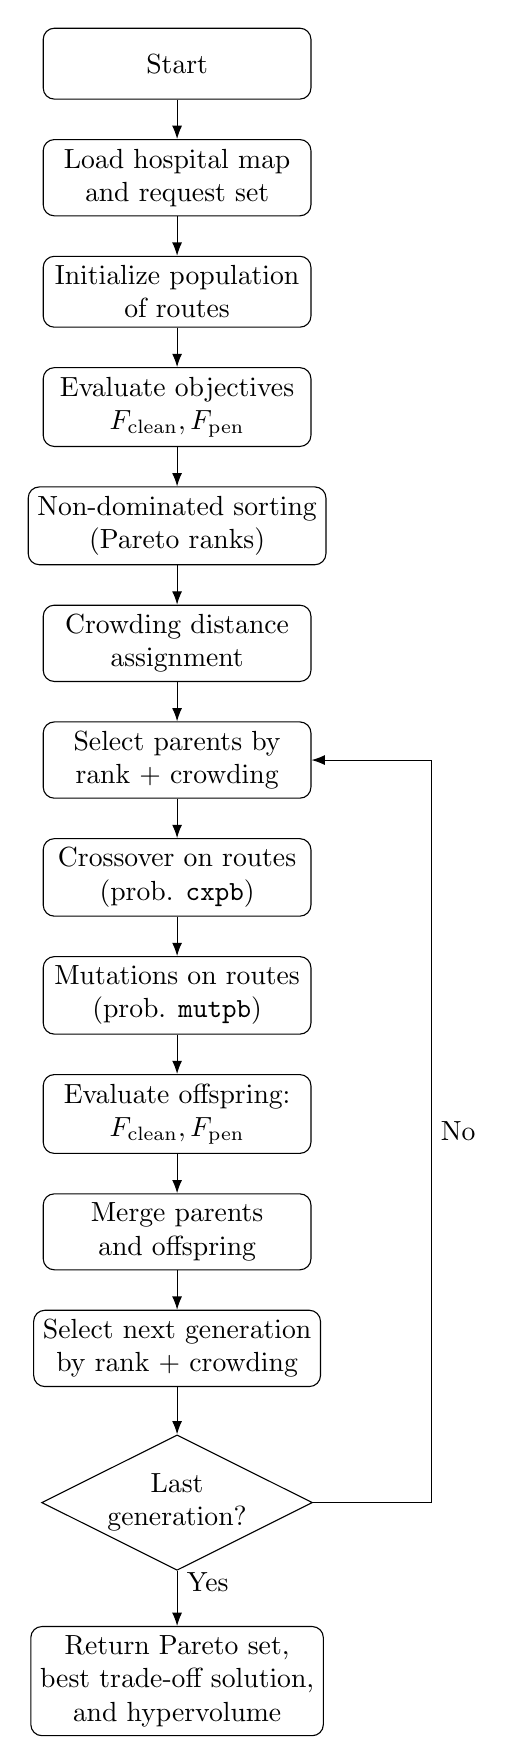
\begin{tikzpicture}[
  node distance=0.5cm,
  >=Latex,
  block/.style={rectangle, draw, rounded corners, align=center, minimum width=3.4cm, minimum height=0.9cm},
  decision/.style={diamond, draw, aspect=2, align=center, inner sep=1pt},
  line/.style={draw, -{Latex}}
]

\node[block] (start) {Start};
\node[block, below=of start] (env) {Load hospital map\\and request set};
\node[block, below=of env] (init) {Initialize population\\of routes};
\node[block, below=of init] (eval) {Evaluate objectives\\$F_{\text{clean}}, F_{\text{pen}}$};
\node[block, below=of eval] (nds) {Non-dominated sorting\\(Pareto ranks)};
\node[block, below=of nds] (crowd) {Crowding distance\\assignment};
\node[block, below=of crowd] (select) {Select parents by\\rank + crowding};
\node[block, below=of select] (crossover) {Crossover on routes\\(prob. \texttt{cxpb})};
\node[block, below=of crossover] (mutation) {Mutations on routes\\(prob. \texttt{mutpb})};
\node[block, below=of mutation] (eval2) {Evaluate offspring:\\$F_{\text{clean}}, F_{\text{pen}}$};
\node[block, below=of eval2] (merge) {Merge parents\\and offspring};
\node[block, below=of merge] (selnext) {Select next generation\\by rank + crowding};
\node[decision, below=of selnext, yshift=-0.1cm] (stop) {Last\\generation?};
\node[block, below=of stop, yshift=-0.2cm] (end) {Return Pareto set,\\best trade-off solution,\\and hypervolume};

\path[line] (start) -- (env);
\path[line] (env) -- (init);
\path[line] (init) -- (eval);
\path[line] (eval) -- (nds);
\path[line] (nds) -- (crowd);
\path[line] (crowd) -- (select);
\path[line] (select) -- (crossover);
\path[line] (crossover) -- (mutation);
\path[line] (mutation) -- (eval2);
\path[line] (eval2) -- (merge);
\path[line] (merge) -- (selnext);
\path[line] (selnext) -- (stop);

\path[line] (stop.east) -- ++(1.5,0) |- (select.east) node[pos=0.25, right]{No};
\path[line] (stop.south) -- (end.north) node[pos=0.2, right]{Yes};

\end{tikzpicture}
\end{document}
